%%%%%%%%%%%%%%%%%%%%%%%%%%%%%%%%%%%%%%%%%%%%%%%%%%%%%%%%%%%%%%%%%%%%%%%%%%%%%%%

\documentclass[12pt,twocolumn,tighten]{aastex62}
%\documentclass[12pt,twocolumn,tighten,trackchanges]{aastex62}
\usepackage{amsmath,amstext,amssymb}
\usepackage[T1]{fontenc}
\usepackage{apjfonts}
\usepackage[figure,figure*]{hypcap}
\usepackage{graphics,graphicx}
\usepackage{hyperref}
\usepackage{natbib}
\usepackage[caption=false]{subfig} % for subfloat

\renewcommand*{\sectionautorefname}{Section} %for \autoref
\renewcommand*{\subsectionautorefname}{Section} %for \autoref

\newcommand{\ptfo}{PTFO$\,$8-8695}
\newcommand{\ptfob}{PTFO$\,$8-8695b}

%% Reintroduced the \received and \accepted commands from AASTeX v5.2.
%% Add "Submitted to " argument.
\received{\today}
\revised{---}
\accepted{---}
\submitjournal{AAS journals.}
\shorttitle{Seeing Double: PTFO$\,$8-8695}

%\objectname{PTFO 8-8695}
%\objectname{PTFO 8-8695b}
%\objectname{CVSO 30}

\begin{document}

\defcitealias{bouma_wasp4b_2019}{B19}

%\title{Against the Planetary Interpretation of PTFO$\,$8-8695b}
% \title{Seeing Double: Still Against the Planetary Interpretation of
% PTFO$\,$8-8695b}
% \title{Seeing Double: TESS and Gaia Show That PTFO$\,$8-8695b is Unlikely a
% Planet}
%\title{Seeing Double: Indications From {\it TESS} and {\it Gaia} That
%PTFO$\,$8-8695b is Not a Planet}
\title{Seeing Double: Transient Dips and Photometric Binarity in
PTFO$\,$8-8695}

\correspondingauthor{L. G. Bouma}
\email{luke@astro.princeton.edu}

%
% key authors:
%
\author[0000-0002-0514-5538]{L. G. Bouma}
\affiliation{ Department of Astrophysical Sciences, Princeton
University, 4 Ivy Lane, Princeton, NJ 08540, USA}
%
\author[0000-0002-4265-047X]{J. N. Winn}
\affiliation{ Department of Astrophysical Sciences, Princeton
University, 4 Ivy Lane, Princeton, NJ 08540, USA}

\begin{abstract}
  PTFO$\,$8-8695b is a candidate hot Jupiter in the 7--10 million year
  old Orion-OB1a cluster. We inspected data from TESS and Gaia to
  clarify whether it is truly a planet.  The Gaia data show that
  PTFO$\,$8-8695 is a photometric binary with respect to members of
  its kinematic group.  The TESS lightcurve shows that the dominant
  variability in this system is a sinusoid with a long period
  $P_{\rm \ell}=11.96\,$hr, presumably caused by stellar rotation.
  Also present is a complex signal, previously identified as the
  planet candidate, that repeats with a short period $P_{\rm s}=
  10.74\,$hr.  The two signals beat every 4.48 days.  Although there
  is a dip in the short-period signal, ground-based photometry from
  the past decade indicates that the orbital phase of the dip seems to
  have instantaneously jumped, at least once, and perhaps twice.
  Planets do not ``jump'' in orbital phase.  Given the available
  evidence, we believe that PTFO$\,$8-8695 is a binary M dwarf in
  which one star shows the long rotation signal, and the other star
  shows ``transient dipping'' that has been seen in a few other young
  weak-lined T Tauri stars.  The origin of these transient dips is
  still undetermined, but our preferred explanation is eclipsing
  clouds of gas or dust at the Keplerian co-rotation radius.
\end{abstract}

\keywords{
	Exoplanet evolution (491),
  Pre-main sequence stars (1290),
	Stellar ages (1581),
	Stellar rotation (1629),
	Variable stars (1761),
  Low mass stars (2050)
}

%%%%%%%%%%%%%%%%%%%%%%%%%%%%%%%%%%%%%%%%%%%%%%%%%%%%%%%%%%%%%%%%%%%%%%%%%%%%%%%

\section{Introduction}
If \ptfob\ were a planet, it would be exceptional.  At below 10
million years of age, it could be the youngest hot Jupiter known
\citep{van_eyken_ptf_2012}.  Its orbital period of only 10.7 hours
around a weak-lined T Tauri M dwarf would also give it the shortest
period of any known hot Jupiter.  With such a short period, it would
almost certainly have filled its Roche lobe, and would be actively
losing mass to its host star.  Not only that, but the rapidly rotating
host star would also be oblate and gravity darkened, and so the
planet's orbit would likely precess into and out of transitability
\citep{barnes_measurement_2013,ciardi_followup_2015,kamiaka_revisiting_2015}. 

Other lines of evidence would imply further planetary ``firsts'' for
this planet candidate.  One first would be that its transits are about
three times deeper in optical bandpasses ({\it e.g.,} $g$-band) than
in the near-infrared ({\it e.g.}, $z$-band)
\citep{onitsuka_multicolor_2017,tanimoto_evidence_2020}.  A cloud-free
hydrogen-dominated planetary atmosphere cannot explain such a
wavelength dependence.  The planet might therefore be surrounded by a
dust cloud \citep{tanimoto_evidence_2020}.  

Another first could be the direct detection of H$\alpha$ emission from
the planet itself \citep{johnskrull_h_2016}.  While the stellar
chromosphere emits in H$\alpha$, it seems that there is an additional
excess H$\alpha$ emission that could be in phase with the planetary
orbit.  The average velocity width of the excess H$\alpha$ emission is
87$\,$km$\,$s$^{-1}$, and its equivalent width is 70-80\% that of the
stellar chromosphere \citep{johnskrull_h_2016}.  The proposed
explanation is that outflowing mass from the planet could explain this
excess emission as well \citep{johnskrull_h_2016}.

There are perhaps a few challenges to the planetary interpretation (if
these ``features'' are not already seen as such).  They include that
the planet does not seem to emit infrared radiation in occulation, at
least at the expected amplitude \citep{yu_tests_2015}.  In
addition, despite measurement attempts by multiple investigators, it
does not seem to show the Rossiter effect at the amplitude expected
given the rapid stellar rotation and large planet size
\citep{yu_tests_2015,ciardi_followup_2015}.  Finally, detailed
modelling of the ``precession + gravity darkening'' transits has shown
that the necessary degree of gravity darkening is too great, given the
spectroscopically observed equatorial velocity
\citep{howarth_reappraisal_2016}.  Additionally, as the
gravity-darkened star precessed about its rotation axis, it would need
to show photometric variability that has not been observed.

While the planetary interpetation clearly faces challenges,
alternative explanations do as well.  High-latitude accretion hotspots
might produce the observed H$\alpha$ variability, and require
fine-tuning produce dips of the approach duration. Furthermore, \ptfo\
does not have an infrared (IR) excess associated with the presence of
an inner disk \citep[{\it e.g.},][Figure~18]{yu_tests_2015}.
Low-latitude starspots, hot or cold, struggle to produce the necessary
dip durations.

Another potential explanation is that between 0.1\% and 1\% of rapidly
rotating low-mass stars in $\mathcal{O}$(10)$\,$Myr old associations
show narrow dips in phase with strong stellar rotation signals
\citep{rebull_usco_2018}.  The dips can persist over months, but their
depths often vary, and sometimes change immediately after stellar
flares.  The explanation proposed by \citet{stauffer_orbiting_2017}
and \citet{david_transient_2017} to explain this novel class of
variable stars is that a circumstellar cloud of dust or gas might be
orbiting near the Keplerian co-rotation radius.  Given available
ground-based data, this explanation is not clearly viable for \ptfo,
because a clear determination of the stellar rotation period has not
yet been possible
\citep{van_eyken_ptf_2012,koen_multicolour_2015,raetz_yeti_2016}.

We begin in Section~\ref{sec:observations} by describing newly
available observations from TESS \citep{ricker_transiting_2015} and
Gaia \citep{gaia_collaboration_gaia_2018}.  The TESS lightcurve shows
two distinct signals, which we extract and analyze in
Section~\ref{sec:tess}.  A long-period sinusoid repeats every 12.0
hours, and is probably stellar rotation.  A short-period dip with an
additional complex modulation repeats every 10.7 hours.  Analyzing the
Gaia data in Section~\ref{sec:gaia}, we show that relative to its
kinematic group, \ptfo\ is a photometric binary.  We collect and
discuss the puzzle pieces in Section~\ref{sec:discussion}.  The
orbital phase of the dip seems to have instantaneously changed over
the past decade.  In addition, a number of other young stars show
lightcurve morphologies similar to the short-period signal.  We
therefore argue that PTFO$\,$8-8695 is a binary M dwarf in which one
star shows a rotation signal, and the other shows ``transient
dipping'' caused by eclipses of material at the Keplerian co-rotation
radius.  Section~\ref{sec:conclusions} summarizes our main points.


\section{The Data}
\label{sec:observations}

\begin{figure*}[t!]
	\begin{center}
		\leavevmode
		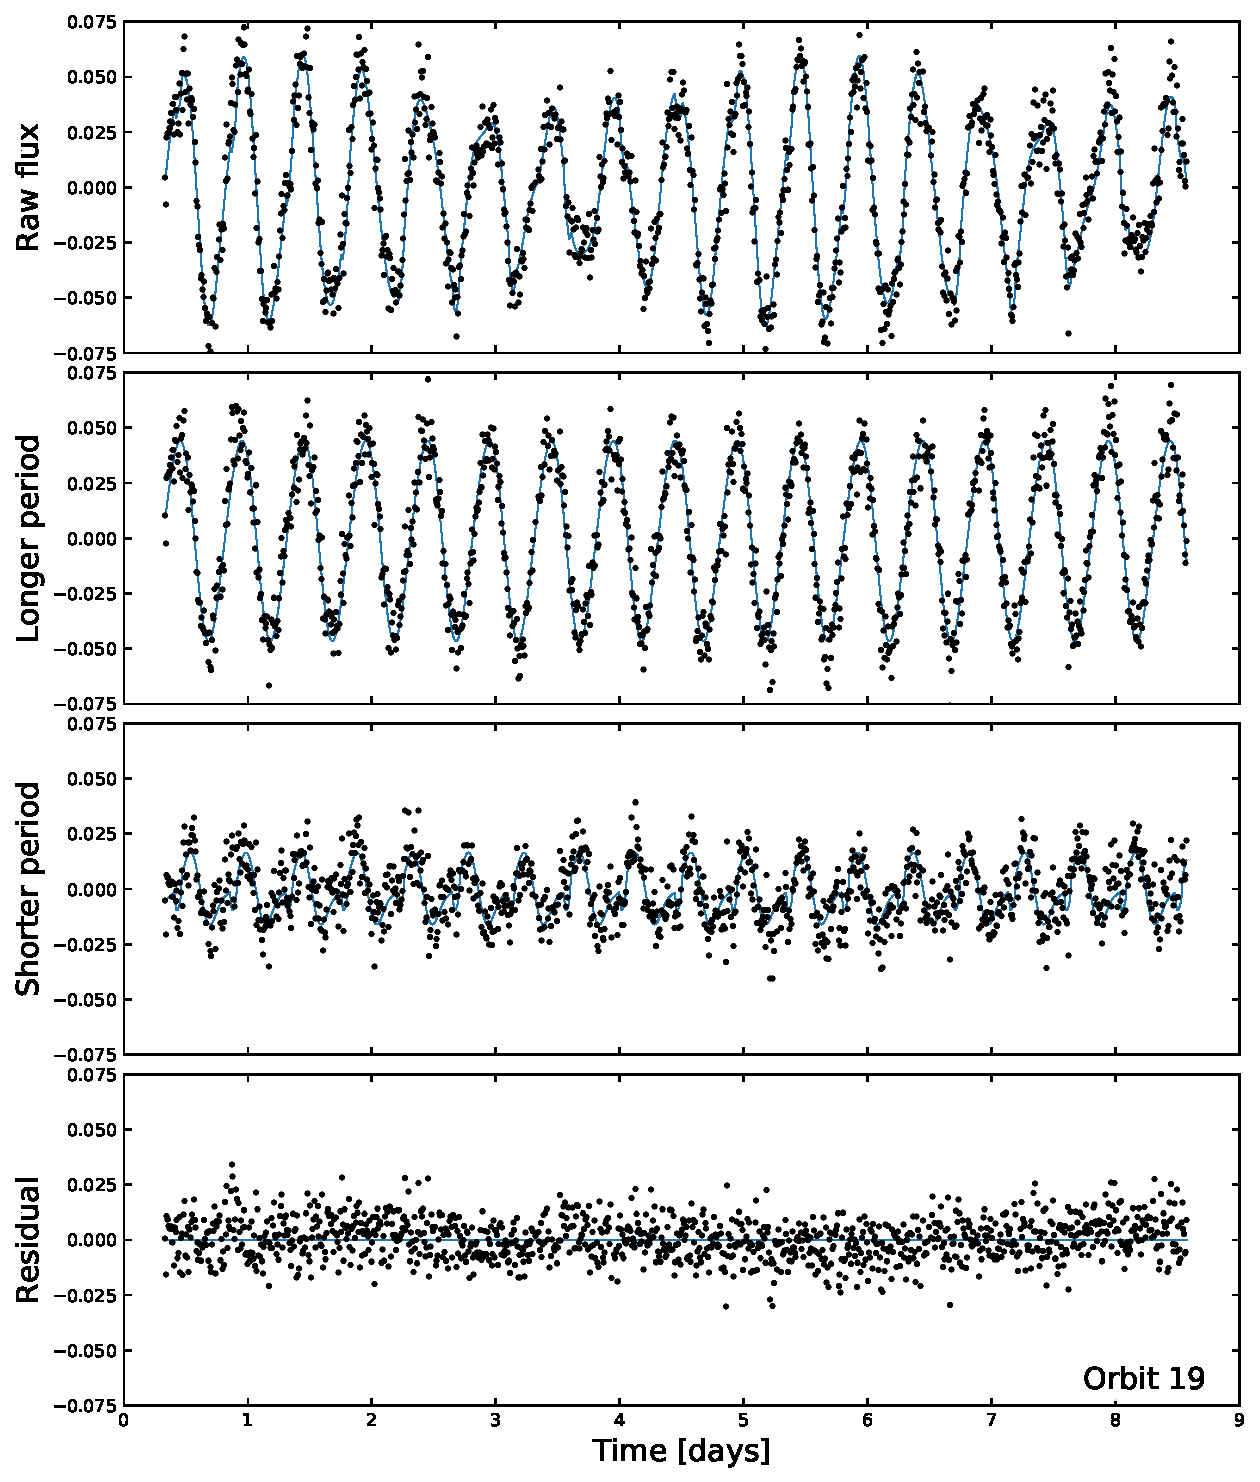
\includegraphics[width=1\textwidth]{f1.pdf}
	\end{center}
	\vspace{-0.7cm}
	\caption{
		{\bf TESS lightcurve of \ptfo\ (Sector 6, Orbit 19).}
    {\it Top}: ``Raw'' \texttt{PDCSAP} mean-subtracted relative flux
    versus time. The beat period of 4.48 days is visible by eye.  The
    preferred model plotted underneath the data includes 2 harmonics
    at the long period $P_{\rm \ell}$, plus 2 harmonics and a transit
    at the short period $P_{\rm s}$.
		{\it Upper middle}: Long-period signal, equal to the raw signal
		minus the short-period signal.
		{\it Lower middle}: Short-period signal, equal to the raw signal
		minus the long-period signal.
		{\it Bottom}: residual.  The data are binned from 2 to 10 minute
		cadence as a convenience for plotting and fitting.
		\label{fig:splitsignal}
	}
\end{figure*}

\begin{figure*}[hbtp]
	\begin{center}
		\leavevmode
		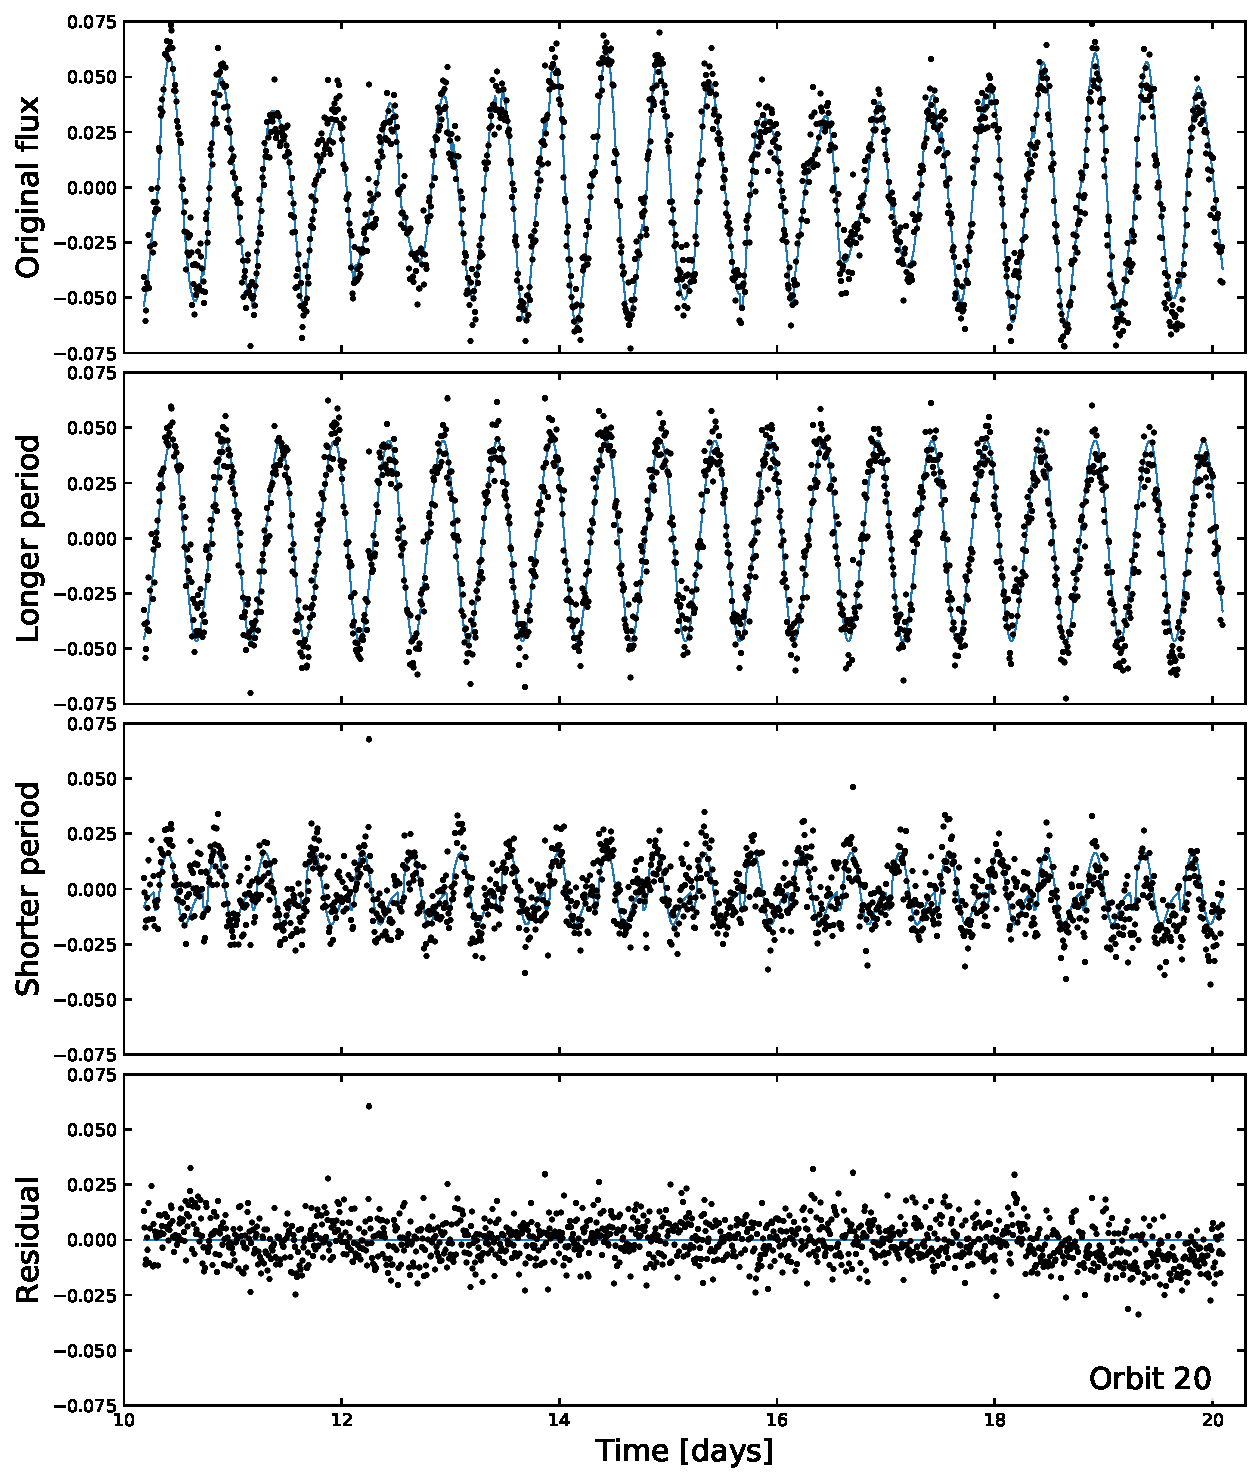
\includegraphics[width=1\textwidth]{f2.pdf}
	\end{center}
	\vspace{-0.7cm}
  \caption{ {\bf TESS lightcurve of \ptfo\ (Sector 6, Orbit 20).}
		Panels are as in Figure~\ref{fig:splitsignal}.
		\label{fig:splitsignalii}
	}
\end{figure*}

\subsection{TESS Observations}

\ptfo\ was observed by TESS with Camera 1, CCD 1, from December 15,
2018 to January 6, 2019, during the sixth sector of science operations
\citep{ricker_transiting_2015}.  The star was designated TIC 264461976
in the TESS Input Catalog \citep{stassun_TIC_2018,stassun_TIC8_2019}.
The pixel data for an $11\times11$ array surrounding \ptfo\ were
averaged into 2-minute stacks by the onboard computer.  Each
2048$\times$2048 image from the CCD was also averaged into 30-minute
stacks, and saved as a ``full frame image'' (FFI).

The 2-minute stacks for \ptfo\ were reduced to lightcurves by the
Science Processing Operations Center (SPOC) at NASA
Ames~\citep{jenkins_tess_2016}.  Our main analysis used the resulting
Presearch Data Conditioning (PDC) lightcurve.  The PDC lightcurve
aperture used pixels chosen to maximize the SNR of the total flux of
the target \citep{smith_kepler_apertures_2017}.  Non-astrophysical
variability was removed through the methods discussed by
\citet{smith_kepler_PDC_2017}.

As an independent check on the shorter cadence SPOC light-curve, we
separately processed the 30-minute image stacks as part of the Cluster
Difference Imaging Photometric Survey (CDIPS;
\citealt{bouma_cluster_2019}).  Our CDIPS lightcurve  of choice used a
circular aperture with radius 1 pixel.

To clean the data, we removed all points with non-zero quality flags
\citep[{\it e.g.},][]{tess_data_product_description_2018}.  We also
masked out the first and last 6 hours of each orbit, since there is
often systematic red noise during those times.  Both the CDIPS and PDC
lightcurves showed a clear discontinuous ``jump'' in the last few days
of orbit 20, which seemed likely to be an instrumental systematic.  We
correspondingly masked out times from BJD 2458488.3 until the end of
the orbit.  The PDC lightcurve initially had 15{,}678 points.  The
quality-flag cut removed 854 points; masking the orbit edges removed an
additional 716; removing the final few days of orbit 20 removed an
additional 1079.  After cleaning, 83\% of the initial flux
measurements remained.

We normalized these points by dividing out the median flux. We opted
to then subtract by unity to simplify subsequent interpretation.  Many
of these and subsequent processing steps were performed using
\texttt{astrobase}~\citep{bhatti_astrobase_2018}. 


\subsection{Gaia Observations}

\subsubsection{Astrometry of \ptfo}

Between July 25, 2014 and May 23, 2016, Gaia measured about 300
billion centroid positions of 1{.}6 billion stars
\citep{gaia_collaboration_gaia_2016,lindegren_gaiasoln_2018,gaia_collaboration_gaia_2018}.
In the Gaia second data release (DR2), these CCD observations were
used to estimate positions, proper motions, and parallax for the
brighest 1{.}3 billion stars, including \ptfo\
\citep{lindegren_gaiasoln_2018}.  There were 121 ``good'' observations
of \ptfo, that is observations that were not strongly down-weighted in
its astrometric solution.  \ptfo\ was assigned a Gaia DR2 identifier
of 3222255959210123904.  It photometric brightness was measured using
selected bands ($G$, $Rp$, and $Bp$) of the Gaia Radial Velocity
Spectrometer \citep{cropper_gaia_2018,evans_gaia_2018}.  We accessed
the pipeline parameters for \ptfo\ using the Gaia
archive\footnote{\url{gea.esac.esa.int/archive/}}.

The majority of Gaia's derived parameters for \ptfo\ agreed with
expectation from former studies
\citep{briceno_cida_2005,van_eyken_ptf_2012}.  One novelty however was
that Gaia DR2 detected a significant ``astrometric excess'', at a
level of 10.3$\sigma$.  We comment on the significance and
interpretation of this excess in Section~\ref{sec:gaia}.


\subsubsection{Hierarchical Cluster Membership}
\label{subsec:hierarchical}

Gaia also provided astrometric parameters for tens of thousands of
young stars in the Orion complex.  Stellar populations in giant
molecular cloud complexes are not monolithic; substructured groups are
the norm \citep{briceno_lowmassOB_2007}.  The Orion molecular cloud
complex in particular has numerous subgroups, with ages spanning 0.5
to 15$\,$Myr. For an incomplete sampling, see for instance
\citet{briceno_cida_2005,jeffries_kinematic_2006,briceno_25_2007,kounkel_apogee2_2018}
and \citet{briceno_cidaII_2019}.

\ptfo\ was initially identified as a member of the Orion$\,$OB1a
sub-association by \citet{briceno_cida_2005} through combined
photometry and spectroscopy.  Later work by \citet{briceno_25_2007}
clarified that \ptfo\ was in a kinematically distinct subgroup of
Orion~OB1a, named the ``25$\,$Ori'' group after its brightest
member. The 25$\,$Ori group had an isochrone age of 7--10$\,$Myr, and
had a smaller disk fraction than younger nearby sub-associations
\citep{hernandez_spitzer_ob1_2007}.

With the Gaia astrometry, it has become clear that 25$\,$Ori itself
has further subgroups
\citep{kounkel_apogee2_2018,briceno_cidaII_2019}.  In describing the
cluster membership of \ptfo, we follow the notation and results of
\citet{kounkel_apogee2_2018}.  These authors combined astrometric data
from Gaia DR2 with near-infrared spectra from APOGEE-2
\citep{gunn_sdss_2006,majewski_apache_2017,blanton_sloan_2017,zasowski_target_2017,cottle_apogee2_2018}.
They performed a hierarchical clustering on the six dimensional
position and velocity information to identify subgroups within the
Orion complex.  From smallest to largest, \ptfo\ was identified
as a member of the following hierarchical subgroups:
\begin{equation}
  %{\rm PTFO\,8\text{-}8695}
  % \in
  {\rm 25\,Ori\text{-}1}
  \subset {\rm 25\,Ori}
  \subset {\rm Orion\ OB1a}
  \subset {\rm Orion\ D},
\end{equation}
where from set-notation, `$\subset$' denotes ``is a proper subset
of''.  25$\,$Ori-1 is the largest subgroup of 25$\,$Ori, with 149
identified members.  Its mean age from its CMD was found to be
6.9$\,$Myr, and from its HR diagram 8.5$\,$Myr
\citep{kounkel_apogee2_2018}.  \citet{kounkel_apogee2_2018} identified
seven other smaller groups in the Orion complex near the Be star
25$\,$Ori. These groups received higher numbers, {\it e.g.},
25$\,$Ori-2 (${\rm Age}_{\rm CMD} =15.1\,$Myr; ${\rm Age}_{\rm CMD}
=12.9\,$Myr; see also \citealt{briceno_cidaII_2019}).

These details concerning the group membership for one object may seem
cumbersome to those accustomed to comparing ``young cluster members''
with ``old field stars''.  Though all members of the Orion complex are
indeed young relative to the field, these details are essential for
assessing any evidence for photometric binarity in \ptfo, because of
the degeneracy between stellar luminosity and age for
pre-main-sequence stars.  Having a clean sample of tightly spatially
and kinematically associated reference stars minimizes contamination
not just from the field, but from older and younger members of the
Orion complex itself.


\section{TESS Analysis}
\label{sec:tess}

\begin{figure*}[t]
	\begin{center}
		\leavevmode
		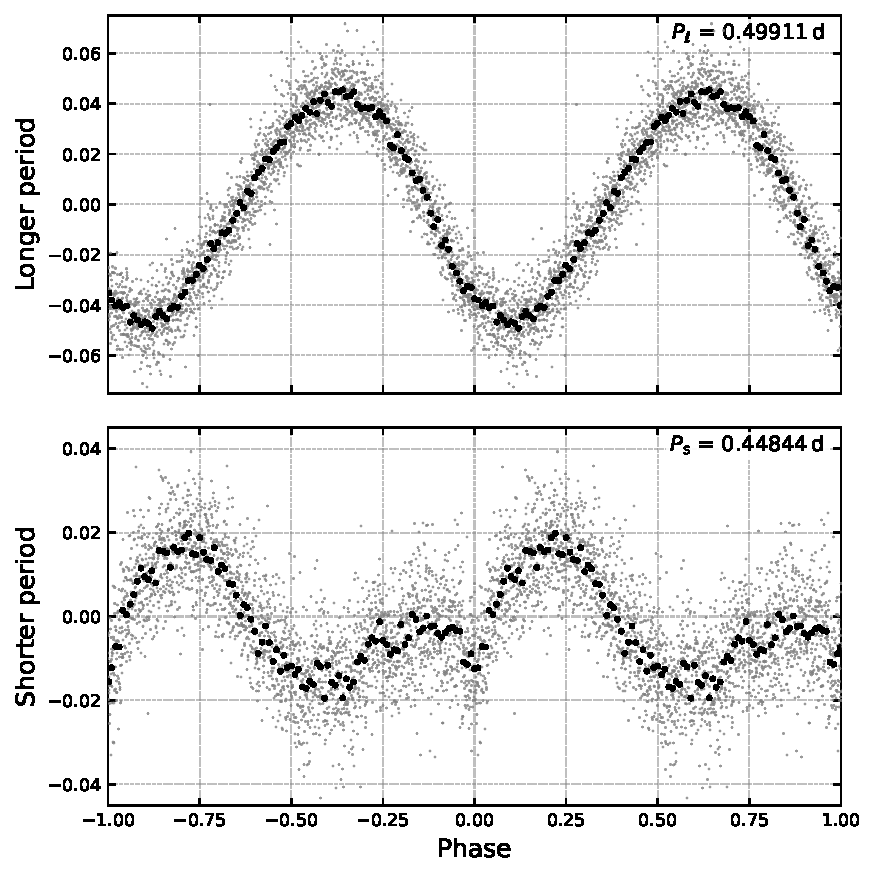
\includegraphics[width=0.99\textwidth]{f3.pdf}
	\end{center}
	\vspace{-0.7cm}
	\caption{ {\bf Phase-folded long and short-period signals.}
    {\it Top}: Long-period signal, as in Figure~\ref{fig:splitsignal}.
    {\it Bottom}: Short-period signal. The reference phase is set to
    the ``planetary'' dip.  Gray points are the 10 minute cadence
    \texttt{PDCSAP} flux.  Black points are binned to 100 points per
    period.
		\label{fig:phasefold}
	}
\end{figure*}

\subsection{Inspection}

Our initial inspection of the TESS lightcurve, in both its 2-minute
PDCSAP and 30-minute FFI forms, showed a strong sinusoidal beat signal
(Figures~\ref{fig:splitsignal} and~\ref{fig:splitsignalii}, top
panel).

As a precursor to more detailed analysis, we calculated generalized
Lomb-Scargle periodograms using \texttt{astrobase}
\citep{lomb_1976,scargle_studies_1982,vanderplas_periodograms_2015,bhatti_astrobase_2018}.
The two largest peaks in the Lomb-Scargle periodogram of the
lightcurve were clearly separated at a ``short'' period $P_{\rm s}
\approx 0.448\,{\rm days}$ and a ``long'' period $P_{\rm \ell} \approx
0.499\,{\rm days}$.  The $P_{\rm \ell}$ peak had the greater power of
the two.  Smaller harmonics surrounding each of these two dominants
peaks were also present.

% 0.14 = A1+A2
% 0.06 = A1-A2
% 2A1 = 0.20
% -> A1 = 0.1
% 2A2 = 0.08
% -> A2 = 0.04

The peak-to-peak lightcurve amplitude at maximum, when the two signals
constructively interfere, is about 14\%.  At minimum, the peak-to-peak
amplitude is about 6\%.  Assuming the signals are just two sinusoids,
algebra tells us that the peak-to-peak amplitudes should therefore be
10\% for the long-period signal, and 4\% for the short-period signal.
These order-of-magnitude numbers will turn out to be roughly correct.

Initial signal-processing experiments fitting out splines or sinusoids
showed that after subtracting out the long-period signal, the
short-period signal dominated the periodogram, and vice-versa.
However it quickly became clear that it would be beneficial to
simultaneously model the signals separately, in order to preserve the
power at each frequency.




\subsection{Lightcurve Model}

We fitted the lightcurve as a linear combination of Fourier harmonics
at the short and long periods, plus a transit at the short period.
Symbolically, the total flux $f$ is given as
\begin{equation}
  f = f_{\rm s} + f_{\rm \ell}
  = f_{\rm transit,s} + f_{\rm Fourier,s} + f_{\rm Fourier,\ell},
\end{equation}
where $f_{\rm s}$ is the relative flux at the short period, and
$f_{\rm \ell}$ is the flux at the long period.  Writing out the
Fourier terms,
\begin{align}
  f = &f_{\rm transit,s} + \sum_{n=1}^{N} A_n \sin(n\omega_{\rm s}t)
  + \sum_{n=1}^{N} B_n \cos(n\omega_{\rm s}t)\\
  &+ \sum_{m=1}^{M} A_m \sin(m[\omega_{\rm \ell}t+\phi_{\rm \ell}])
  + \sum_{m=1}^{M} B_m \cos(m[\omega_{\rm \ell}t+\phi_{\rm \ell}]), \nonumber
\end{align}
for $N$ and $M$ the total number of harmonics at the short and long
periods, respectively, $A_i$ and $B_i$ the amplitudes for each
harmonic term (potentially negative), and $\omega_i = 2\pi / P_i$ the
angular frequency for $i$ the short or long period index.  We fixed
the ``phase-offset'' for the short period signal to be zero, and let
the reference time for the long period signal float by introducing
$\phi_{\rm \ell}$.  Since we did not a priori know how many harmonics
would be appropriate, we considered a number of different choices for
$N$ and $M$, and used the Bayesian information criterion to choose the
appropriate model (Table~1).

As an example, one possible model could be a transit, plus $N=2$
harmonics of sines and cosines at the short period, plus $M=1$
harmonics at the long period.  For this case the free parameters would
be as follows.  For the transit, we would fit for the impact
parameter, the planet-to-star radius ratio, two quadratic limb
darkening parameters, the planet orbital period (equal to the short
period), the reference time for the transit, and the mean flux.  There
would be $2N=4$ additional Fourier amplitudes at the short period,
plus $2M=2$ Fourier amplitudes at the long period, and well as the
long period itself and its phase.  For this case, we therefore fitted
14 free parameters.

We implemented and fitted the models using \texttt{PyMC3}, which is
built on \texttt{theano}
\citep{salvatier_2016_PyMC3,exoplanet:theano}.  For the Fourier terms,
we used the default math operators.  For the exoplanet transit, we
used the model and derivatives implemented in \texttt{exoplanet}
\citep{exoplanet:exoplanet}.  Our priors are listed in Table~2.  To
speed up the fitting, we re-sampled the cleaned 2 minute lightcurves
to 10 minute binning.  We correspondingly scaled the uncertainties in
the flux measurements by a factor of $\sqrt{5}$.  Before sampling, we
initialized each model to the maximum a posteriori (MAP) solution.  We
then sampled using \texttt{PyMC3}'s gradient-based No-U-Turn Sampler
\citep{hoffman_no-u-turn_2014}, and used $\hat{R}$ as our convergence
diagnostic \citep{gelman_inference_1992}.  We tested our ability to
successfully recover injected parameters using synthetic data, before
fitting the \ptfo\ lightcurves.


\subsection{Fitting Results}

We considered nine models, with the number of harmonics per frequency
$N$ and $M$ ranging from one to three.  To select our preferred model,
we used the Bayesian information criterion (Table~1).  The model with
the lowest BIC had two harmonics at the short 10.74$\,$hr period, and
two harmonics at the long 11.96$\,$hr period.  The next-best model had
an additional harmonic at the longer period ($M=3$), but was otherwise
identical.  All nine models have reduced $\chi^2$ ranging between 1.37
and 1.51, which suggests a plausible though imperfect agreement
between the data and fitting results.  The best-fit parameters for the
lowest BIC model are given in Table~2.

To explore where each model succeeded and failed, we split the raw
signal into its respective components (Figures~\ref{fig:splitsignal}
and~\ref{fig:splitsignalii}).  We also examined the phase-folded
signals (Figure~\ref{fig:phasefold}).  

In every model, the $11.96\,{\rm hr}$ variability is a simple sinusoid
with peak-to-peak amplitude $\approx$10\%.  The $10.74\,{\rm hr}$
variability is always more complex.  A dip of depth $\approx$1.2\%,
fit in our model as a transit, lasts $\approx$0.75 hours.  Superposed
on the dip is a slightly asymmetric sinusoid with peak-to-peak
amplitude of about 4\%. The asymmetric sinusoid peaks near phase 0.25,
and reaches minimum brightness between phases -0.5 and -0.25.  The
flux at phase $\approx -0.33$ shows what could be a discontinuous
jump, shortly after reaching minimum (Figure~\ref{fig:phasefold}).
This jump was visible in each of the nine models we considered.

The periodogram of the final residual (Figure~\ref{fig:splitsignal}
bottom row) shows a weakly significant, poorly resolved peak at
$\approx$8 days, consistent with the visual impression in the time
domain that there could be a weak long-period signal present.



\section{Binarity Analysis}
\label{sec:gaia}

\subsection{Visual Binarity}
\label{subsec:blend}

\begin{figure}[t]
	\begin{center}
		\leavevmode
		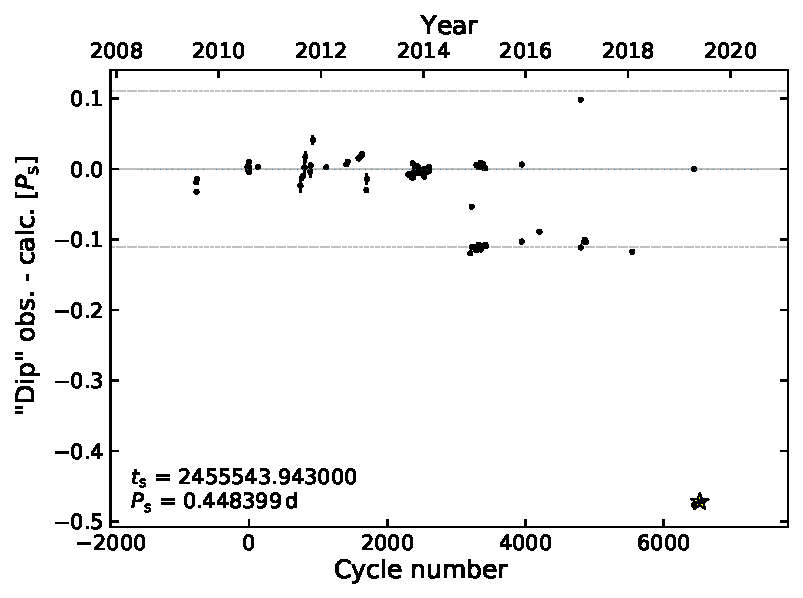
\includegraphics[width=0.45\textwidth]{f4.pdf}
	\end{center}
	\vspace{-0.7cm}
	\caption{ {\bf Scene used for blend analysis.}
		{\it Top:} Mean TESS image of \ptfo\ over Sector~6, with a
		log-stretch.  The position of \ptfo\ is shown with a yellow
		star.  Neighbors with $T<17$ are shown with orange crosses.  The
		apertures used to measure the background and target star flux are
		shown with \texttt{X} and \texttt{/} hatches, respectively.
		{\it Bottom:} Digitized Sky Survey $R$-band image of the same
		field, with a linear stretch. The circles show apertures of radii
		1, 1.5, and 2.25 pixels used in part of our blend analysis.  The
		pixel level TESS data show that ``Star A''  does not contribute
		variability at either of the two observed periods (see
		Section~\ref{subsec:blend}).
		\label{fig:scene}
	}
\end{figure}


The TESS pixels are $\approx21$'' per side. Before making any
interpretations, we needed to consider whether light from known
neighboring stars could have affected the photometry.  The scene is
shown in Figure~\ref{fig:scene}.  In the upper panels, the pixels used
to measure the background level in the SPOC lightcurve are indicated
with an `\texttt{X}' hatch, and the pixels used in the final
lightcurve aperture are shown with the `\texttt{/}' hatch.

The target star, \ptfo\ (TIC 264461976), has a $T$-band magnitude of
14.0, and its position is shown with a star.  The other (unlabeled)
star inside the target aperture, TIC 264461979, has $T=16.8$ and so
cannot contribute a signal with relative amplitude 10\%.  The only
neighbor that is sufficiently close and bright that its light might
contaminate the target star is TIC 264461980, with $T=14.8$, which we
dub ``Star A''.  Star A is 23.6'' NW of our target, and based on the
magnitude difference could contribute up to 48\% the flux of our
target star, \ptfo.  

Because \ptfo\ was previously identified to have periodicity
consistent with our measurement of $P_{\rm s}$, our main concern
regarding blending was the degree to which we could be certain that
the long-period signal at $P_{\rm \ell}$ also originated from \ptfo.
We took two approaches to verifying the source of the long-period
signal.

First, we examined the CDIPS FFI lightcurves of the target, which were
available on MAST \citep{bouma_cluster_2019}.  The maximal
peak-to-peak beat amplitude was constant across apertures of radii 1,
1.5, and 2.25 pixels to visual precision ($\lesssim 1\%$).  If Star A
were the source of the long-period variability, we would expect the
peak variability amplitude to be smallest in the 1 pixel aperture,
based on the separation of the sources (Figure~\ref{fig:scene},
bottom).  From this test alone, it seems unlikely that Star A is the
source of the long-period signal.

Second, we examined the 2-minute lightcurve of each pixel in the scene
individually.  We opted to use the interactive tools implemented in
\texttt{lightkurve} \citep{lightkurve_2018}.  If Star A were the
source of the long-period variability, we would expect the pixels
nearest to Star A to show a sinusoidal signal with amplitude exceeding
$10\%$.  The data do not support this possibility.  The pixel directly
below Star A does not clearly show the sinusoidal variability, and the
peak-to-peak variability in that pixel is $\lesssim 8\%$.  In
contrast, the south-easternmost pixel within \ptfo's aperture (the
pixel furthest from Star A that was used in the optimal aperture)
shows the $P_{\rm \ell}$ sinusoidal variability signal at $\approx
14\%$ amplitude.  We conclude that within the resolution of the Gaia
DR2 source catalog, the $P_{\rm s}$ and $P_{\rm \ell}$ signals
originate from \ptfo.  From \citet{ziegler_measuring_2018}, we can
surmise that stellar companions wider than $\approx$1'' (349~AU) and
within $\Delta G \approx 3$ magnitudes of \ptfo\ would have likely
been detected through this approach. 

\citet{van_eyken_ptf_2012} obtained stronger constraints on possible
stellar companions using the NIRC2 camera on Keck II.  They reported
3$\sigma$ $H$-band magnitude difference limits of 4.3, 6.4, and 8.9 at
angular separations of 0.25, 0.5, and 1.0 arcseconds (87, 175, and
349~AU).  They also detected a point-source, not present in Gaia DR2,
7.0 magnitudes fainter than the target, and 1.8$''$ north-east.  Due
to the brightness difference, this coincident star\footnote{This
companion was claimed to be a potential planetary-mass object
\citep{schmidt_direct_2016}. Subsequent analysis of its colors showed
that it is a background star \citep{lee_evidence_2018}.} cannot be the
source of our signals.


%FIXME: would be better to actually be able to get them...
While long-baseline radial velocity measurements could provide
complimentary lower limits on companion masses and separations, the RV
data for \ptfo\ are rather poor owing to the stellar faintness.  The
longest single-instrument baseline in the literature appears to be 5
Keck/HIRES measurements acquired over 10 days in April 2011 by
\citet{van_eyken_ptf_2012}.  The RV RMS over that 10 day span was
$1.6\,{\rm km}\,{\rm s}^{-1}$, consistent with the measurement
precision.  Though \citet{yu_tests_2015} acquired 22 further
Keck/HIRES observations over one night in December 2013, these points
seem to not have been reduced to velocities.  Further Keck/HIRES
measurements of this target could confirm or refute the existence of
possible binary companions.



\subsection{Photometric Binarity}

\begin{figure*}[t]
	\begin{center}
		\leavevmode
		\subfloat{
			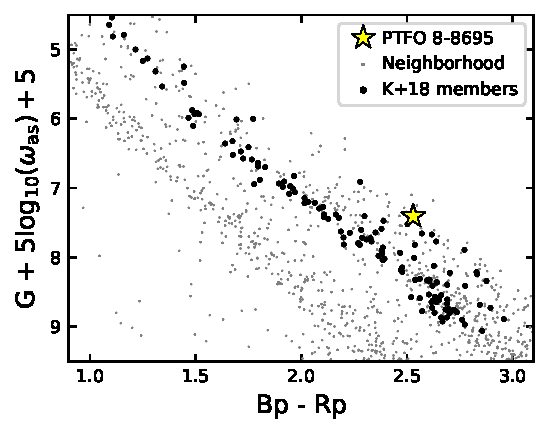
\includegraphics[width=0.7\textwidth]{f5a.pdf}
		}
		
		\vspace{-0.7cm}
		\subfloat{
			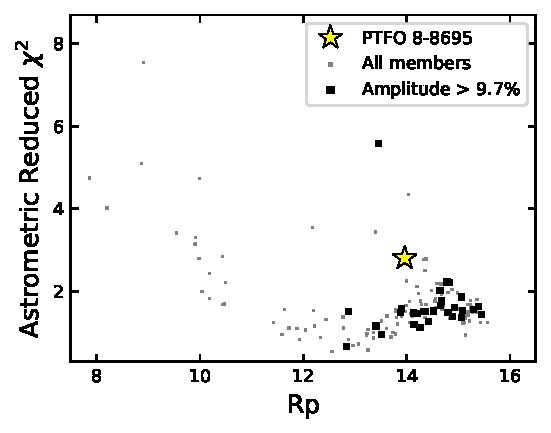
\includegraphics[width=0.7\textwidth]{f5b.pdf}
		}
	\end{center}
	\vspace{-0.7cm}
	\caption{ {\bf Evidence for binarity in \ptfo}.
    {\it Top: Hertzsprung-Russell diagram of \ptfo\ and late-type
    members of 25$\,$Ori-1.} Members of the 25$\,$Ori-1 group (black
    circles) were identified by \citet{kounkel_apogee2_2018} through
    clustering on six-dimensional Gaia DR2 and APOGEE-2 data.  The
    ``neighborhood'' (gray circles) is non-member stars within 5
    standard deviations of the mean 25$\,$Ori-1 right ascension,
    declination, and parallax.  It contains members of the Orion
    complex with its full spread of ages, in addition to field
    interlopers.  $G$ denotes Gaia broadband magnitudes, $Bp$ Gaia
    blue, $Rp$ Gaia red, and $\omega_{\rm as}$ the parallax in
    arcseconds.  The $x$-axis limits have been set to show only K and
    M dwarf members, to accentuate \ptfo's separation from the
    single-star sequence.  {\it Bottom: Astrometric goodness-of-fit
    versus $Rp$ magnitude for 25$\,$Ori-1 members}.  The single-source
    astrometric model for \ptfo\ provides a poor fit, which could be due to
    stellar variability or binarity.  Cluster members that
    are at least as variable as \ptfo\ show lower astrometric excesses
    (black squares), suggesting binarity as the root cause.
		\label{fig:gaia}
	}
\end{figure*}


Aside from visual binarity, we can also check the Gaia data for
photometric binarity.  To assemble a set of stars coeval with \ptfo,
we used the 25$\,$Ori-1 members identified by
\citet{kounkel_apogee2_2018}, and discussed in
Section~\ref{subsec:hierarchical}.

To define a set of non-member stars that nonetheless had comparable
selection functions, we defined a reference ``neighborhood'' as the
group of at most $10^4$ randomly selected non-member stars within 5
standard deviations of the mean 25$\,$Ori-1 right ascension,
declination, and parallax.  We queried Gaia DR2 for these stars using
\texttt{astroquery} \citep{astroquery_2018}.  This yielded 1{,}819
neighbors.  While some of these stars may indeed be members of the
Orion complex, or even of 25$\,$Ori-1, enforcing this cut on positions
and parallaxes ensures that we are querying stars with comparable
amounts of interstellar reddening.

We examined the resulting five-dimensional right ascension,
declination, proper motions, and parallaxes.  The first point we noted
was that 25$\,$Ori-1 was a clearly defined over-density in each
dimension---the cluster exists, and is distinct from the neighborhood.
\ptfo\ was also within the cluster in each of these projected
dimensions.

Given our detection of two separate signals, whether \ptfo\ could be a
photometric binary was of great interest.  Figure~\ref{fig:gaia} shows
the HR diagram we constructed to assess this issue.  The diagram shows
that \ptfo\ is $\approx$0.75 magnitudes brighter than the average
25$\,$Ori-1 star of the same color.  In other words, it is about twice
as bright.  It also seems to be coincident with the photometric binary
track of the cluster, which has a few other stars.

The implication is that either {\it (i)} \ptfo\ is notably younger
than the kinematically identical 25$\,$Ori-1 members, or {\it (ii)}
\ptfo\ is a photometric binary.  Since there is no a priori reason to
suspect an age difference, but we have resolved two separate
photometric signals, the binary interpretation seems somewhat more
likely.


\subsection{Astrometric Binarity}

A separate possible line of evidence for binarity is the Gaia DR2
astrometry.  As noted in Section~\ref{sec:observations}, the Gaia DR2
solution for \ptfo\ shows a 10.3$\sigma$ astrometric excess.  This
astrometric excess indicates the degree to which a single-source model
fails to explain the observed astrometric measurements.  Specifically,
the single-source astrometric model yielded $\chi^2=325.2$.  There are
121 astrometric measurements, and 5 free parameters, and therefore 116
degrees of freedom. The reduced $\chi^2$ is 2.80.  The majority of
stars with comparable brightness in Gaia do not show such poor
goodness-of-fit \citep[see][Appendix A]{lindegren_gaiasoln_2018}.

Potential explanations for the poor astrometric fit include
photometric variability and unresolved stellar binarity \citep[{\it
e.g.},][]{rizzuto_ZEIT8_2018,belokurov_unresolved_2020}.  If
photometric variability were the cause, we would expect comparably
faint stars in the same kinematic group of Orion to show similar
astrometric excesses, as the majority of young stars are highly
variable.

% NB: CDIPS-I only made 131 light-curves for 25Ori-1, because I wasn't
% aware of the Kounkel+18 member list at the time.
Using the same 149 members in the 25$\,$Ori-1 subgroup, we calculated
the astrometric reduced $\chi^2$ for each member.  We then queried the
CDIPS lightcurve database at MAST \citep{bouma_cluster_2019} to find
the subset of stars that were at least as variable as \ptfo.
We measured the variability amplitude by taking the difference of the
$95^{\rm th}$ and $5^{\rm th}$ percentiles of the flux.
This yielded 30 stars of equal or greater variability.
The lower panel of Figure~\ref{fig:gaia} shows the
reduced $\chi^2$ as a function of stellar brightness.  \ptfo\ is in
the upper 90$^{\rm th}$ percentile of stars showing astrometric
excesses within the 25$\,$Ori-1 group.  Relative to other M-dwarf
group members with comparable brightnesses and variability
characteristics, \ptfo\ still stands out as behaving astrometrically
poorly.  Ultimately, we will have to wait for the full release of the
nominal Gaia mission to definitively determine whether the astrometric
excess is caused by stellar binarity or photometric variability.
Nonetheless the fact that comparably variable stars do not show
comparably large astrometric excesses suggests that stellar binarity
is indeed the root cause.


\section{Discussion}
\label{sec:discussion}

\subsection{Long period sinusoid}

The standard interpretation for 11.96$\,$hour sinusoidal modulations
of a pre-main-sequence M dwarf is stellar rotation.  This is the
dominant signal in the system with 10\% amplitude, and there is no
evidence to suggest that this signal has any other origin.

The discovery study by \citet{van_eyken_ptf_2012} saw an alias of the
same signal ({\it e.g.}, their Figure~7), and identified it as a
periodogram peak at $0.9985 \pm 0.0061\,$days. They ascribed it to
their observing cadence, because of its close correspondence to the
sidereal day.  While the TESS data can show significant reflected
light from the Earth \citep[{\it e.g.},][]{luger_tess_2019}, our
pixel-level analysis showed that the signal is specific to only pixels
near \ptfo, and no other pixels.  We therefore conclude that the
signal is not a systematic.

We are not the first to reach the conclusion that the long period
sinusoidal modulation is astrophysical.  A study by
\citet{koen_multicolour_2015} identified the same modes and aliases as
\citet{van_eyken_ptf_2012}, but argued that the signal was
astrophysical (however they were still unsure of the exact period).
Using photometry from the YETI global telescope network,
\citet{raetz_yeti_2016} eventually came to the conclusion that the
$0.50\,{\rm d}$ signal was indeed from stellar rotation.  The TESS
data strongly support this conclusion.



\subsection{Short period dip}

\begin{figure}[t]
	\begin{center}
		\leavevmode
		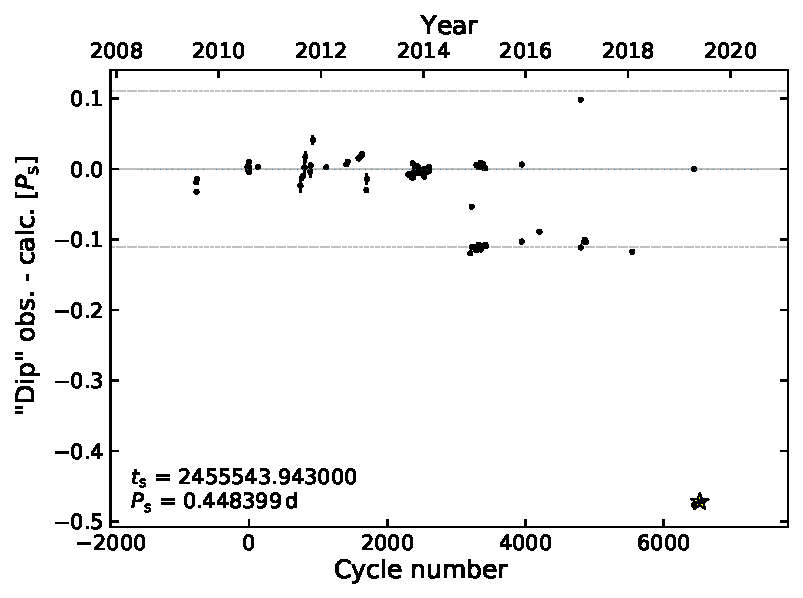
\includegraphics[width=0.5\textwidth]{f6.pdf}
	\end{center}
	\vspace{-0.7cm}
	\caption{
		{\bf Timing residuals for \ptfob\ from a decade of monitoring.}
		Black points are times of dips, minus the indicated linear
		ephemeris.  The $y$-axis is given in units of phase for the
		short-period signal.  The star shows the binned TESS ephemeris.
		Dips have been observed by \citet{van_eyken_ptf_2012},
		\citet{ciardi_followup_2015}, \citet{yu_tests_2015},
		\citet{raetz_yeti_2016}, \citet{onitsuka_multicolor_2017}, and
		\citet{tanimoto_evidence_2020}.  Certain dips ({\it e.g.}, the one
		at phase 0 in mid-2019) are consistent with noise, and were likely
		reported because something was {\it expected}, rather than
		convincingly {\it observed}.  Horizontal dashed lines are drawn at
		$\pm (P_{\rm \ell} - P_{\rm s})/P_{\rm s}$, highlighting either a
		numerical coincidence or an observational bias.  The orbital phase
		observed by TESS (lower-right) is consistent with that of
		\citet{tanimoto_evidence_2020}, and quite different from the
		original phase.
		\label{fig:o_minus_c}
	}
\end{figure}

The TESS lightcurve shows a dip that lasts about 45 minutes, and seems
to re-occur every 10.74 hours
(Figures~\ref{fig:splitsignal},~\ref{fig:splitsignalii},~\ref{fig:phasefold}).
The dip duration is roughly the same as that observed by previous
investigators \citep{van_eyken_ptf_2012,yu_tests_2015}.  The 1.2\%
depth is similar to what has been observed in the near-infrared
\citep{onitsuka_multicolor_2017}.  However the dip depth seems likely
to have evolved over time between being not present at all, to a
maximum of $\approx$5\% \citep[{\it
e.g.},]{koen_multicolour_2015,yu_tests_2015,tanimoto_evidence_2020}.

One particularly interesting feature of the dip is its epoch.  Over
the past decade, many investigators have observed \ptfo.  Its dips do
not always occur on a perfectly linear ephemeris
\citep{yu_tests_2015}.  In fact, \citet{tanimoto_evidence_2020}
recently provided stark evidence for different behavior altogether:
over a time-span of years, the dip ``splits'' into distinct groups at
particular repeating phases.  See for instance their Figures~2
through~4.  Fitting a decade of observations, they provided the
following linear ephemeris, which we did not find any need to update.
\begin{align}
t_0\ {\rm BJD}_{\rm TDB} &= 2455543.943 \pm 0.002 \\
P &= 0.4483993 \pm 0.0000006 d.
\end{align}

In Figure~\ref{fig:o_minus_c}, we show the phase of the dip we detect
in the TESS data, relative to their ephemeris.  It agrees with the
independent December 2018 measurements by
\citet{tanimoto_evidence_2020}: the dip has drastically shifted phase
over the past decade.

Figure~\ref{fig:o_minus_c} shows two additional strange features: {\it
(i)}  multiple dips per cycle, and {\it (ii)} a set of dips
numerically coincident with phase $(P_{\rm \ell} - P_{\rm s}) / P_{\rm
s}$.  The observation of multiple dips per cycle in 2015 was seen
independently by both \citet{yu_tests_2015} and
\citet{tanimoto_evidence_2020}.  It therefore seems credible.
Inspecting the \citet{tanimoto_evidence_2020} lightcurves, the claim
of multiple dips per cycle in December 2018 at phase 0 and -0{.}47
seems less plausible---the phase -0{.}47 dips are strongly detected,
while the suggested phase 0 dip is not clearly present in the data.

We are not sure what to make of the numerical coincidence.  The ratio
of long to short periods is roughly 10:9.  It is not clear that this
would obviously translate into an observational bias unless by some
fluke three season's worth of observations managed to only observe
every ninth dip.  This is of course not the case, and we therefore
leave this curiosity as observation {\it sans} interpretation.



\subsection{Short period out-of-dip modulation}

Visually, the out-of-dip modulation at the 10.74$\,$hour period
resembles a slightly asymmetric sinusoid (Figure~\ref{fig:phasefold}).
Non-zero contributions in both the first and second harmonics are
detected (Table~2).  The first sine and cosine harmonic both have
amplitudes of roughly $0.9\pm0.1\%$.  The second sine harmonic has
amplitude $0.16 \pm 0.07\%$, so is non-zero at a significance of only
2.3$\sigma$.  The second cosine harmonic has negative amplitude $0.53
\pm 0.06\%$.  In our sign convention, the fact that it is negative
means that this component peaks at phase 0.25 and 0.75.

\subsubsection{Planetary interpretation}
If there were a giant planet transiting \ptfo, it would tidally
distort the host star, and cause ellipsoidal photometric modulations
that also peak at quadrature \citep[see][]{shporer_astrophysics_2017}.
Interpreting the second cosine harmonic as planet-induced tidal distortion,
it would imply a minimum planet mass $M_{\rm p} \sin i$ of
$3.8\,M_{\rm Jup}$.  For this estimate, we assumed $R_\star = 1.39
R_\odot$, and $M_\star = 0.39 M_\odot$ \citep{van_eyken_ptf_2012}.
This ellipsoidal amplitude is larger than the typical
modulations induced by close-in giant planets because the host star is
puffy, and still on the pre-main-sequence.

The planetary interpretation however does not readily explain the
first sine and cosine harmonics.  Interpreting the sine component as
Doppler beaming would imply a secondary mass greater than the primary
($0.86\,M_\odot$).  Interpreting the cosine component as reflected or
emitted light from the planet's surface is nonsensical because the sign is wrong---the
planet would need to be {\it absorbing} light.

\subsubsection{Similar Lightcurves}

\begin{figure*}[hbtp]
	\begin{center}
		\leavevmode
		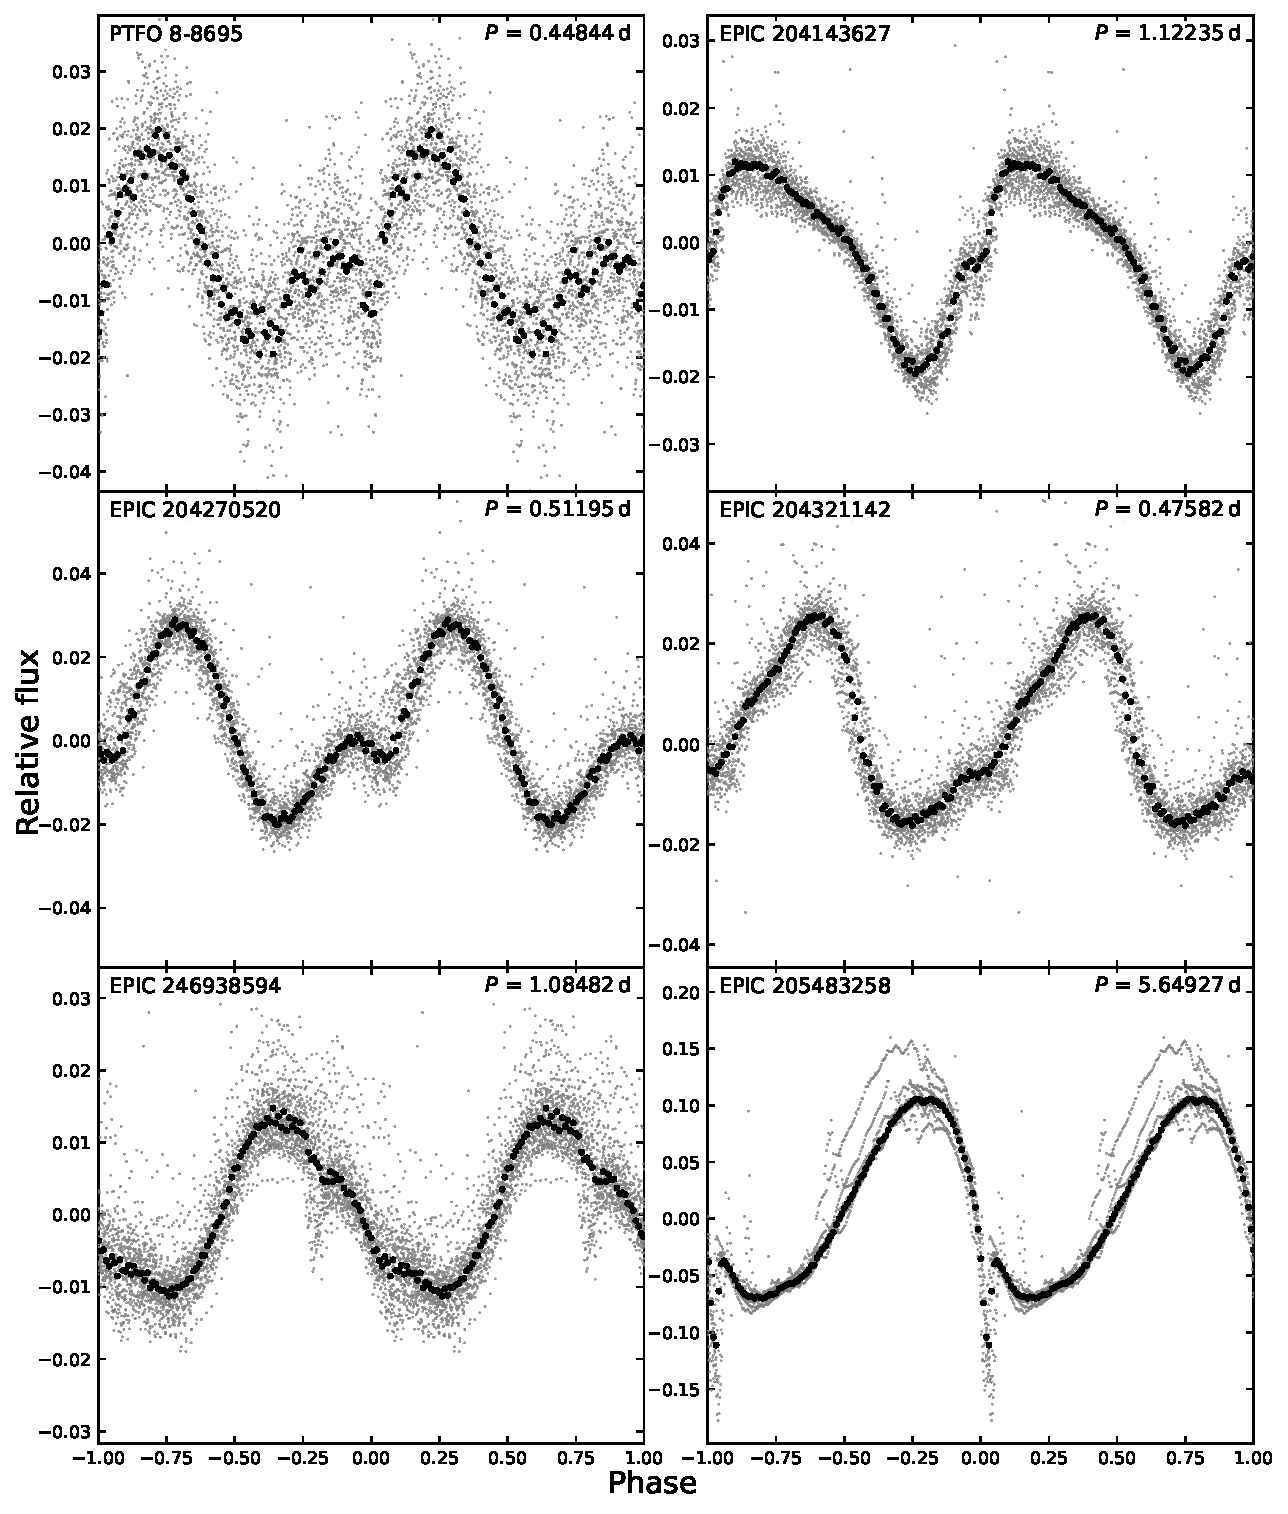
\includegraphics[width=1\textwidth]{f7.pdf}
	\end{center}
	\vspace{-0.7cm}
  \caption{ {\bf \ptfo\ and its brethren.}
    Five transient and persistent flux dip stars selected based on
    their visual similarity to the short-period signal in \ptfo are as
    shown.  They include EPIC 204143627, EPIC 204321142, EPIC
    204270520, EPIC 205483258 (RIK-210), and EPIC 204787516.  RIK-210
    has the longest period of any of these objects.  EPIC 204787516
    has a less angular dip, and could also be an eclipsing binary.
    All stars have similar properties as \ptfo, but are in Upper~Sco.
    We found these objects through studies by
    \citet{stauffer_orbiting_2017}, \citet{david_transient_2017}, and
    \citet{rebull_usco_2018}.
		\label{fig:brethren}
	}
\end{figure*}

When physical explanations are not forthcoming, taxonomy can be a
useful exercise.  To our knowledge, of order 10-20 lightcurves with
similar morphologies have been seen in surveys of low-mass weak-lined
T Tauri stars in regions including $\rho$ Oph, Upper~Sco, Taurus, and
perhaps the Pleiades
\citep{rebull_rotation_2016,david_transient_2017,stauffer_orbiting_2017,stauffer_rotevol_2018,rebull_usco_2018,rebull_rotation_2020}.
These surveys were performed using K2 \citep{howell_k2_2014}.  We
downloaded a few of these lightcurves from MAST, opting for the
EVEREST reductions \citep{luger_everest_2016,luger_update_2018}.  They
are plotted in Figure~\ref{fig:brethren}.

These lightcurves have been phenomenologically classified as
``persistent flux dips'' or ``transient flux dips'', based on whether
their depths and durations show variability over the 90-day K2
campaigns \citep{stauffer_orbiting_2017}.
As \citet{stauffer_orbiting_2017} explain,
these  objects are morphologically distinct from ``scallop shell' lightcurves,
and are present in stars at more advanced evolutionary disk stages than
the ``dipper'' stars \citep{ansdell_young_2016,cody_manyfaceted_2018}.
The persistent and transient flux dip stars have the following properties.
\begin{enumerate}
  \item Weak-lined T Tauri stars.
  \item Spectral type typically M2-M5 ({\it e.g.},
    \citealt{rebull_usco_2018},~Figure~20).
  \item Ages $\lesssim$ 100$\,$Myr.
  \item Stars typically lack spectroscopic accretion indicators 
  \item Phased lightcurves show shallow, angular dips, usually
    superposed on large-amplitude smooth variability. The latter
    is interpreted as stellar rotation.
  \item Rotation is fast---usually between 0.5 and 2.0 days.
  \item Rarely any infrared excess (never any W4 detection; only a few
    cases with W3 detctions).
  \item Can show multiple dips per cycle ({\it e.g.}, EPIC 203692610,
    RIK-210).
  \item Dip depths, durations, and phases can vary over just a few cycles
    ({\it e.g.}, EPIC 204143627).
  \item Dip depths can change after flares.
  \item Rare at a population level: $\lesssim 1\%$ of relevant stars
    \citep{rebull_usco_2018}.
\end{enumerate}
The 10.74 hour signal in \ptfo\ meets all of these criteria.
This is the first connection of \ptfo\ with this class of objects
because the TESS lightcurve was needed to resolve the different
rotation signals.

There are two crucial additional points concerning the transient flux
dips.  First, the dip durations seem to scale linearly with their
periods \citep[][Figure~26]{stauffer_orbiting_2017}.  In the usual
idealized limits, the transit duration $T$ of a point source across
the stellar disk scales as $T \propto R_\star (P/M_\star)^{1/3}$
\citep{winn_exoplanet_2010}.  While the shortest period
$\approx$0.5-day transient flux dip stars have dip durations
consistent with point sources, at longer periods of 1 to 5 days the
dip durations become many hours, and far too long for a point-source
origin.

Second, between 40-50\% of the transient flux dip stars discovered in
$\rho$~Oph and Upper~Sco show two
Lomb-Scargle periods, and so are apparently binaries
\citep[][Table~1]{stauffer_orbiting_2017}.
This is higher than the corresponding main-sequence companion
fraction of ${\rm CF}_{0.1\text{-}0.5\,M_\odot}^{\rm MS} = 33 \pm 5\%$
\citep{henry_solar_2006,duchene_stellar_2013}.
Low-mass pre-main-sequence stars however have been shown to 
companion fractions up to twice as high in dispersed clusters such as
Upper~Sco and Taurus \citep{kraus_mapping_2008,kraus_mapping_2011}.
A detailed high-resolution imaging survey would be necessary to determine
whether the transient flux dip stars truly have any distinct
population-level binarity properties relative to other young low-mass
stars.






\section{Physical Interpretation}

The evidence for binarity in \ptfo\ is as follows.  First, the star is
photometrically twice as bright as stars of the same color in its
kinematic group (Figure~\ref{fig:gaia}.  Second, it shows two distinct
photometric signals.  These points alone suggest binarity
\citep{stauffer_rotevol_2018}.  For the case of \ptfo, there is a
third line of evidence: the Gaia astrometry shows a poor
goodness-of-fit to a single-source model.  While this could be caused
by an additional companion or stellar variability, cluster members
that are equally if not more variable still show \ptfo\ to be an
outlier.  Therefore the astrometric excess is a suggestive third line
of evidence for binarity in \ptfo.  We take these three points
combined to imply that \ptfo\ is probably a binary.

Based on the lack of an infrared excess seen by \citet{yu_tests_2015},
the primordial gas disks seem to be have been depleted\footnote{A
potential confounding factor is completeness. Is Spitzer sensitive to
infrared excesses at the distance of Orion? The series of studies by
\cite{hernandez_spitzer_2006,hernandez_spitzer_ob1_2007,hernandez_spitzer_sig_2007,hernandez_spitzer_2009}
show that it is.} around both stars in \ptfo. The stars are therefore
no longer magnetically locked to their disks.  This is consistent with
the $\approx$half-day periodicities of both rotation signals: young
disked M dwarfs typically rotate with periods of two days or more due
to magnetic locking \citep[{\it e.g.},][]{rebull_rotation_2020}.  If
the two stars are within $\approx$50$\,$AU of each other, as required
by the NIRC2 adaptive optics imaging, then it would also be expected
that the stars would truncate the outer edges of their respective
disks, in a manner seen at the population level in exoplanetary
systems \citep{kraus_impact_2016,moe_impact_2019}.  This hard outer
boundary condition could propagate to the inner disk and affect its
evolution.

The main physical question remaining is clearly what causes the
transient dipping. This is an unsolved problem not only for \ptfo\ but
also for an emerging class of similar young rapidly rotating M-dwarfs.
Some possible explanations are highly disfavored, for reasons that
have been detailed by \citet{david_transient_2017},
\citet{stauffer_orbiting_2017}, and \citet{zhan_complex_2019}.
These disfavored explanations include that the dips are caused by
{\it (i)} eclipsing binaries;
{\it (ii)} ``dipper''-flavor Class-I or Class-II disks;
{\it (iii)} eclipses of prominences;
{\it (iv)} high-latitude accretion hotspots;
{\it (v)} high-latitude starspots;
and
{\it (vi)} dust clouds of reasonable composition.
We also view the possibility of {\it (vii)} tidally disrupted planetary
or cometary material to be implausible, given the synchronicity
between dip and rotation periods, and the stability of signals
observed in some systems.

The explanations that are not yet ruled out include
{\it (i)} transiting clumps of gas at the Keplerian corotation radius;
{\it (ii)} transits of enshrouded protoplanets;
{\it (iii)} occultations of starspots by an optically thick disk.
The first and last explanations offer added appeal because they are
flexible enough to explain not only the transient and persistent-dip
M-dwarfs, but also the ``scallop shell'' M-dwarfs
\citep{stauffer_orbiting_2017}.
Despite this appeal, the possibility of distinct mechanisms 
explaining these
distinct variability classes should remain open.


\section{Conclusions}
\label{sec:conclusions}

\ptfo\ was previously thought to potentially host a hot Jupiter.
The TESS lightcurve of \ptfo\ showed a number of new features,
many of which seem to disfavor the hot Jupiter interpretatation.
The TESS data showed two key pieces of evidence.
\begin{enumerate}
  \item {\it Two periodic signals.} The ``long'' signal is a 10\%
      peak-to-peak sinusoidal modulation repeating every 11.96 hours.
      The ``short'' signal is a 4\% peak-to-peak complex modulation
      repeating every 10.74 hours. It is composed of a dip, plus at
      least two harmonics. The signals beat, and therefore cannot be
      an artifact linked to data processing.
  \item {\it A dip at the wrong orbital phase.} The clearest dip in
    the ``short'' signal was consistent with recent observations by
    \citet{tanimoto_evidence_2020}, and differed from the discovery
    epoch by 5.14 hours.
\end{enumerate}

The physical mechanism responsible for all these features remains a
matter of speculation.
With that said, the TESS data support new arguments against the planetary
interpretation of \ptfo.
First, if the long signal is caused by starspot modulation, and the
short signal by a transiting planet, what causes the additional
complex modulations seen at the short, ``orbital'', period?

Given the available evidence,
PTFO$\,$8-8695 seems consistent with the
``transient dipping'' phenomenology observed in many young M dwarfs.
Though it seems rather unlikely to be a planet, understanding \ptfo\
and its analogs will help us understand the natal environments 
of the majority of Earth-sized planets in the Milky Way
\citep{dressing_occurrence_2013}.



%%%%%%%%%%%%%%%%%%%%%%%%%%%%%%%%%%%%%%%%%%%%%%%%%%%%%%%%%%%%%%%%%%%%%%%%%%%%%%%

% \acknowledgements
% %
% This paper includes data collected by the TESS mission, which are
% publicly available from the Mikulski Archive for Space Telescopes
% (MAST).
% %
% Funding for the TESS mission is provided by NASA's Science Mission
% directorate.
% %
% This work made use of NASA's Astrophysics Data System Bibliographic
% Services.
% %
% Based on observations obtained at the Gemini Observatory, which is
% operated by the Association of Universities for Research in Astronomy,
% Inc., under a cooperative agreement with the NSF on behalf of the
% Gemini partnership: the National Science Foundation (United States),
% National Research Council (Canada), CONICYT (Chile), Ministerio de
% Ciencia, Tecnolog\'{i}a e Innovaci\'{o}n Productiva (Argentina),
% Minist\'{e}rio da Ci\^{e}ncia, Tecnologia e Inova\c{c}\~{a}o (Brazil),
% and Korea Astronomy and Space Science Institute (Republic of Korea).
% %
% Observations in the paper made use of the High-Resolution Imaging
% instrument Zorro at Gemini-South. Zorro was funded by the NASA
% Exoplanet Exploration Program and built at the NASA Ames Research
% Center by Steve B. Howell, Nic Scott, Elliott P. Horch, and Emmett
% Quigley.
% %
% This research has made use of the VizieR catalogue access tool, CDS,
% Strasbourg, France. The original description of the VizieR service was
% published in A\&AS 143, 23.
% %
% This work has made use of data from the European Space Agency (ESA)
% mission {\it Gaia} (\url{https://www.cosmos.esa.int/gaia}), processed
% by the {\it Gaia} Data Processing and Analysis Consortium (DPAC,
% \url{https://www.cosmos.esa.int/web/gaia/dpac/consortium}). Funding
% for the DPAC has been provided by national institutions, in particular
% the institutions participating in the {\it Gaia} Multilateral
% Agreement.
%
% (Some of) The data presented herein were obtained at the W. M. Keck
% Observatory, which is operated as a scientific partnership among the
% California Institute of Technology, the University of California and
% the National Aeronautics and Space Administration. The Observatory was
% made possible by the generous financial support of the W. M. Keck
% Foundation.
% The authors wish to recognize and acknowledge the very significant
% cultural role and reverence that the summit of Maunakea has always had
% within the indigenous Hawaiian community.  We are most fortunate to
% have the opportunity to conduct observations from this mountain.
%
% \newline
%

\software{
  \texttt{astrobase} \citep{bhatti_astrobase_2018},
  % \texttt{astroplan} \citep{astroplan2018},
  \texttt{astropy} \citep{astropy_2018},
  \texttt{astroquery} \citep{astroquery_2018},
  % \texttt{BATMAN} \citep{kreidberg_batman_2015},
  \texttt{corner} \citep{corner_2016},
  %\texttt{emcee} \citep{foreman-mackey_emcee_2013},
  \texttt{exoplanet} \citep{exoplanet:agol19}
  \texttt{exoplanet} \citep{exoplanet:exoplanet}, and its
  dependencies \citep{exoplanet:agol19, exoplanet:kipping13, exoplanet:luger18,
  	exoplanet:theano}.
  \texttt{IPython} \citep{perez_2007},
	\texttt{lightkurve} \citep{lightkurve_2018},
  \texttt{matplotlib} \citep{hunter_matplotlib_2007}, 
  \texttt{MESA} \citep{paxton_modules_2011,paxton_modules_2013,paxton_modules_2015}
  \texttt{numpy} \citep{walt_numpy_2011}, 
  \texttt{pandas} \citep{mckinney-proc-scipy-2010},
  \texttt{PyMC3} \citep{salvatier_2016_PyMC3},
  \texttt{radvel} \citep{fulton_radvel_2018},
  % \texttt{scikit-learn} \citep{scikit-learn},
  \texttt{scipy} \citep{jones_scipy_2001}.
}


% \facilities{
% 	{\it Astrometry}:
% 	Gaia \citep{gaia_collaboration_gaia_2016,gaia_collaboration_gaia_2018}.
% 	{\it Imaging}:
% 	Gemini:South~(Zorro; \citealt{scott_nessi_2018}.
% 	{\it Spectroscopy}:
% 	Keck:I~(HIRES; \citealt{vogt_hires_1994}),
% 	Euler1.2m~(CORALIE),
% 	ESO:3.6m~(HARPS; \citealt{mayor_setting_2003}).
% 	{\it Photometry}:
% 	CTIO:1.0m (Y4KCam),
% 	Danish 1.54m Telescope,
% 	El Sauce:0.356m,
% 	Elizabeth 1.0m at SAAO,
% 	Euler1.2m (EulerCam),
% 	Magellan:Baade (MagIC),
% 	Max Planck:2.2m	(GROND; \citealt{greiner_grond7-channel_2008})
% 	NTT,
% 	SOAR (SOI),
% 	TESS \citep{ricker_transiting_2015},
% 	TRAPPIST \citep{jehin_trappist_2011},
% 	VLT:Antu (FORS2).
% }

%
% The following are entries from Table 1 that are not otherwise cited
% in the text
%
% \nocite{wilson_wasp-4b_2008}
% \nocite{gillon_improved_2009}
% \nocite{winn_transit_2009}
% \nocite{hoyer_tramos_2013}
% \nocite{dragomir_terms_2011}
% \nocite{sanchis-ojeda_starspots_2011}
% \nocite{nikolov_wasp-4b_2012}
% \nocite{ranjan_atmospheric_2014}
% \nocite{huitson_gemini_2017}

% \input{WASP-4b_transit_time_table.tex}
% \input{WASP-4b_rv_table.tex}
% \input{model_fit_table.tex}
% \input{rv_model_posterior_table.tex}
% \input{pdot_table.tex}

\clearpage
\startlongtable
\begin{deluxetable*}{lrrrrrrrr}
%
%\tabletypesize{\scriptsize}
%
\tablenum{1}
%
\tablecaption{Model Comparison.}
\label{tab:modelcompare}
%
\tablehead{
\colhead{Description} &
\colhead{$N_{\rm s}$} &
\colhead{$N_{\rm \ell}$} &
\colhead{$N_{\rm data}$} &
\colhead{$N_{\rm param}$} &
\colhead{$\chi^2$} &
\colhead{$\chi_{\rm red}^2$} &
\colhead{BIC} &
\colhead{$\Delta$BIC}
}
% pasted from
% /Users/luke/Dropbox/proj/billy/results/PTFO_8-8695_results/20200413_v0/bic_table_data.tex
\startdata
Favored    & 2 &  2 &   2585 &      17 &  3523.6 &     1.372 &  3657.2 &    0.0 \\
\hline
Somewhat favored & 2 &  3 &   2585 &      19 &  3512.7 &     1.369 &  3662.0 &    4.8 \\
\hline
Disfavored        & 3 &  2 &   2585 &      19 &  3543.1 &     1.381 &  3692.4 &   35.2 \\
---        & 3 &  3 &   2585 &      21 &  3536.8 &     1.379 &  3701.9 &   44.6 \\
---        & 1 &  2 &   2585 &      15 &  3680.0 &     1.432 &  3797.9 &  140.7 \\
---        & 1 &  3 &   2585 &      17 &  3670.2 &     1.429 &  3803.8 &  146.6 \\
---        & 2 &  1 &   2585 &      15 &  3700.9 &     1.440 &  3818.8 &  161.6 \\
---        & 3 &  1 &   2585 &      17 &  3710.2 &     1.445 &  3843.7 &  186.5 \\
---        & 1 &  1 &   2585 &      13 &  3872.7 &     1.506 &  3974.8 &  317.6 \\
\enddata
%
\tablecomments{
	$N_{\rm s}$ and $N_{\rm \ell}$ are the number of harmonics at the short and long periods, respectively.
	$N_{\rm data}$ is the number of fitted flux measurements.
	$N_{\rm param}$ is the number of free parameters in the model.
	The Bayesian information criterion (BIC) and the difference from the maximum $\Delta {\rm BIC}$ are also listed.
}
\vspace{-1cm}
\end{deluxetable*}

% Table of best fit parameters
\startlongtable
\begin{deluxetable*}{llrrrr}
%
\tablecaption{ Best-fit model priors and posteriors. }
\label{tab:posterior}
%
%\tabletypesize{\scriptsize}
%
\tablenum{2}
%
\tablehead{
  \colhead{Param.} & 
  \colhead{Prior} & 
  \colhead{Mean} & 
  \colhead{Std{.} Dev.} &
  \colhead{3\%} &
  \colhead{97\%}
}
% /Users/luke/Dropbox/proj/billy/results/PTFO_8-8695_results/20200413_v0/posterior_table_clean.tex
\startdata
$P_{\rm s}$ & $\mathcal{N}(0.4485; 0.0010)$ & 0.4484732 & 0.0000857 & 0.4483170 & 0.4486367 \\
$t_{\rm s}^{(1)}$ & $\mathcal{N}(0.438096; 0.0020)$ & 0.4384733 & 0.0017440 & 0.4349337 & 0.4415021 \\
$R_{\rm p}/R_\star$ & $\mathcal{N}(0.1100; 0.0033)$ & 0.11 & 0.00308 & 0.10452 & 0.11599 \\
$b$ & $\mathcal{U}(0; 1+R_{\mathrm{p}}/R_\star)$ & 0.7736 & 0.0756 & 0.6346 & 0.8993 \\
$u_1$ & (2) & 0.683 & 0.477 & 0.001 & 1.546 \\
$u_2$ & (2) & 0.004 & 0.417 & -0.793 & 0.727 \\
Mean & $\mathcal{U}(-0.01; 0.01)$ & -0.000885 & 0.000440 & -0.001745 & -0.000088 \\
$\omega_{\rm s}$ & $2\pi/P_{\mathrm{s}}$ & 14.01017 & 0.00268 & 14.00506 & 14.01505 \\
$A_{\mathrm{s},0}$ & $\mathcal{U}(-0.02; 0.02)$ & 0.008903 & 0.000705 & 0.007569 & 0.010277 \\
$B_{\mathrm{s},0}$ & $\mathcal{U}(-0.02; 0.02)$ & 0.009985 & 0.000751 & 0.008504 & 0.011289 \\
$A_{\mathrm{s},1}$ & $\mathcal{U}(-0.02; 0.02)$ & 0.001649 & 0.000696 & 0.000331 & 0.002884 \\
$B_{\mathrm{s},1}$ & $\mathcal{U}(-0.02; 0.02)$ & -0.005267 & 0.000606 & -0.006491 & -0.004203 \\
$\phi_{\rm \ell}$ & $\mathcal{U}(1.3721; 2.1575)$ & 1.74324 & 0.22254 & 1.38274 & 2.08874 \\
$\omega_{\rm \ell}$ & $\mathcal{N}(12.6054; 0.1261)$ & 12.588581 & 0.002040 & 12.584940 & 12.592450 \\
$A_{\mathrm{\ell},0}$ & $\mathcal{U}(-0.06; 0.06)$ & 0.037785 & 0.005150 & 0.028728 & 0.045214 \\
$B_{\mathrm{\ell},0}$ & $\mathcal{U}(-0.06; 0.06)$ & 0.022288 & 0.008592 & 0.008066 & 0.0359 \\
$A_{\mathrm{\ell},1}$ & $\mathcal{U}(-0.02; 0.02)$ & 0.002326 & 0.000756 & 0.000857 & 0.003658 \\
$B_{\mathrm{\ell},1}$ & $\mathcal{U}(-0.02; 0.02)$ & -0.002197 & 0.000744 & -0.003512 & -0.000743 \\
\enddata
%\tablenotetext{}{ 240000 links saved}
\tablenotetext{}{
  (1) To convert mean TESS mid-transit time to ${\rm BJD}_{\rm TDB}$, add 2458468.2.
  (2) Quadratic limb-darkening prior from \citet{exoplanet:kipping13}, implemented by \citet{exoplanet:exoplanet}.
}
\vspace{0cm}
\end{deluxetable*}

\clearpage

\bibliographystyle{yahapj}                            
\bibliography{bibliography} 


\listofchanges

\end{document}
